\documentclass[12pt,a4paper]{article}
\usepackage{graphicx}

\title{Praktikum Physik - Tr\"agheitsmoment}
\author{Simon Marti, Patricia Schwab, Mirco Kocher}
\date{02.03.2012}

\begin{document}
\maketitle

%%
% Ziel
%%
\section*{Ziel}
Berechnung der Tr\"agheitsmomente unterschiedlicher K\"orper durch Messung der Schwingungsperiode und Verifizierung des Satzes von Steiner.

%%
% Motivation
%%
\section*{Motivation}
Der Versuch des Tr\"agheitsmoments eignet sich gut als Einstieg ins Physikpraktikum. Ausserdem kann mit den gemessenen Daten eine umfassende Fehlerrechnung durchgef\"uhrt werden.

%%
% Theorie
%%
\section*{Theorie}
% Tr\"agheitsmoment -------> bruchemer äue ni
% \[  J = \sum{mr^2} \]
Das Tr\"agheitsmoment $J_{Quader}$ eines homogenen Quaders der Masse $m$ mit Lange $l$ und Breite $b$ ist durch folgende Formel gegeben:
\[ J_{Quader} = \frac{m}{12}(l^2 + b^2) \]
Das Tr\"agheitsmoment $J_{Zylinder}$ eines homogenen Zylinders der Masse $m$ mit Radius $R$ und H\"ohe $h$ ist durch folgende Formel gegeben:
\[  J_{Zylinder} = \frac{m}{12}(h^2 + 3R^2) \]
Die Rotationsenergie $E_{rot}$ eines beliebigen K\"orpers mit Tr\"agheitsmoment $J$ und Winkelgeschindigkeit $\omega$ ist durch folgende Formel gegeben:
\[ E_{rot} = \frac{1}{2}J\omega^2 \]
Der Drehimpuls $L$ bei einem Tr\"agheitsmoment von $J$ und Winkelgeschwindigkeit $\omega$ ist durch folgende Formel gegeben:
\[ L = J\omega \]
Das Tr\"agheitsmoment $J$ eines beliebigen K\"orpers bei einer Periodenschwingungsdauer von $T$ und Federkonstante $k$ ist durch folgende Formel gegeben:
\[ J = \frac{T^2k}{4\pi^2} \]

%%
% Experiment
%%
\section*{Experiment}

% Aufbau und Ablauf
\subsection*{Aufbau und Ablauf}
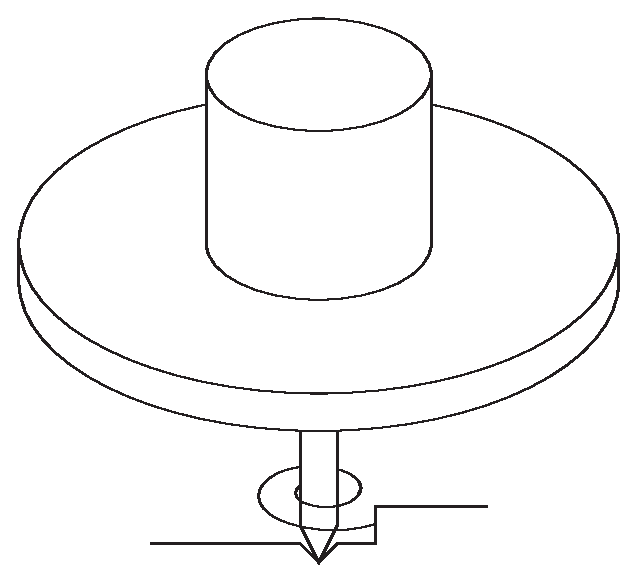
\includegraphics[width=6cm]{illustration11.pdf}

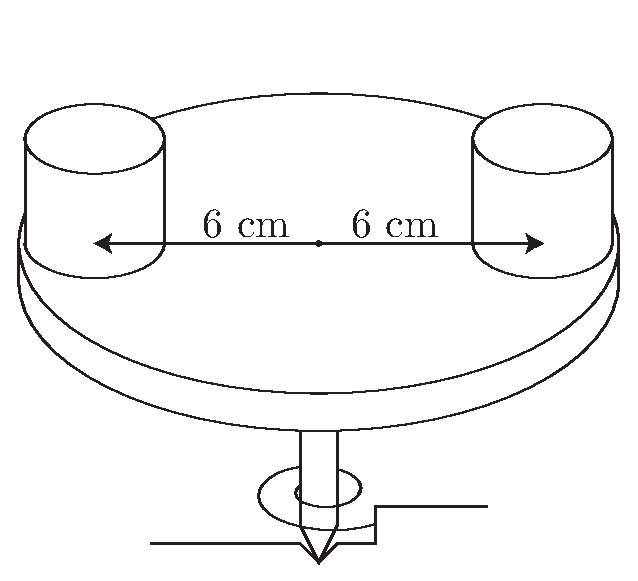
\includegraphics[width=6cm]{illustration12.pdf}

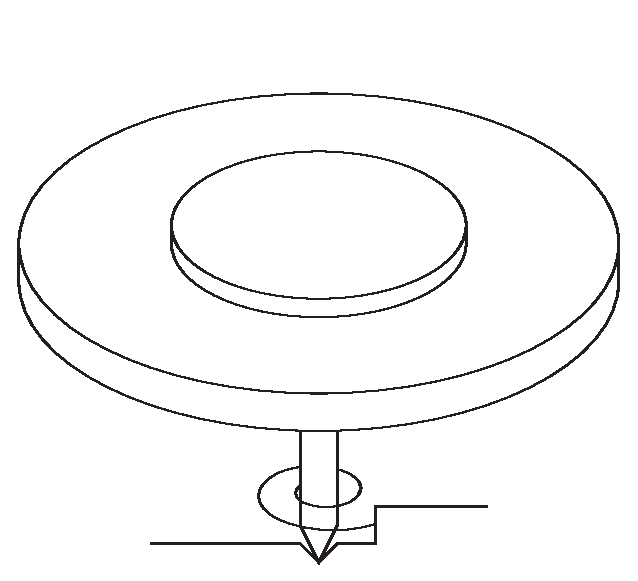
\includegraphics[width=6cm]{illustration21.pdf}

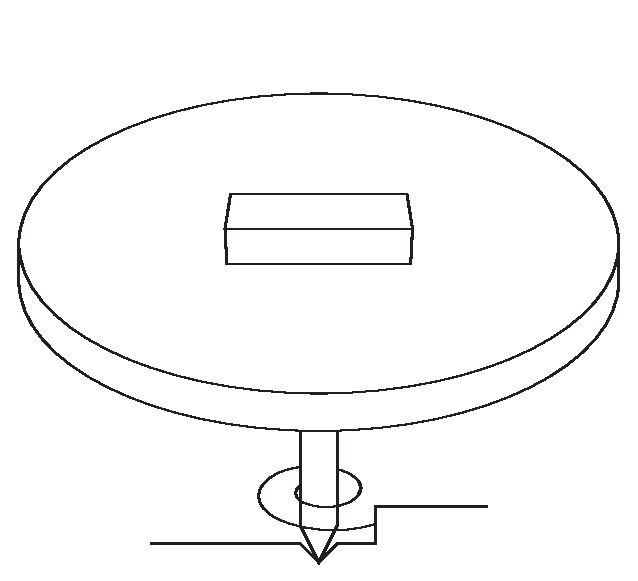
\includegraphics[width=6cm]{illustration22.pdf}

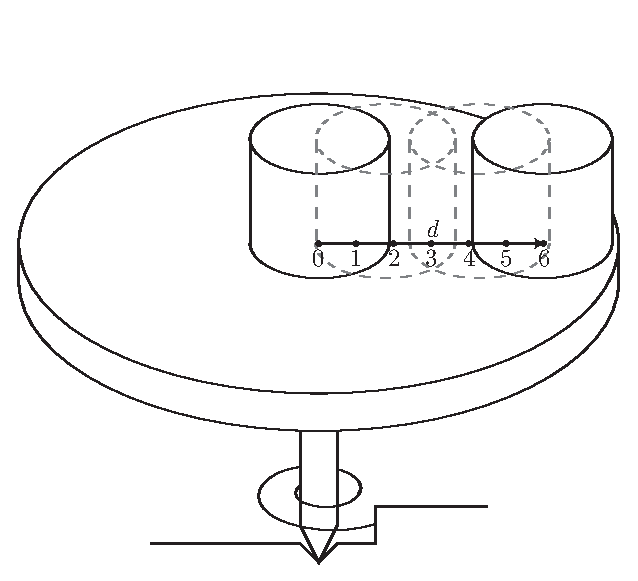
\includegraphics[width=10cm]{illustration3.pdf}

% Rohdaten
\subsection*{Rohdaten}

\begin{tabular}{|l|r|r|r|r|r|r|}
\hline
$d$&$T_1$&$T_2$&$T_3$&$T_4$&$T_5$&$10\overline{T}$\\
\hline
0&12.4 s&12.3 s&12.4 s&12.65 s&12.45 s&12.44 s\\
1&12.55 s&12.7 s&12.75 s&12.7 s&12.55 s&12.65 s\\
2&12.4 s&13.55 s&13.25 s&13.4 s&13.25 s&13.17 s\\
3&14.5 s&14.5 s&14.4 s&14.5 s&14.5 s&14.48 s\\
4&16 s&15.8 s&15.8 s&16 s&16.05 s&15.93 s\\
5&17.6 s&17.55 s&17.7 s&17.65 s&17.5 s&17.60 s\\
6&19.35 s&19.5 s&19.7 s&19.45 s&19.45 s&19.49 s\\
\hline
\end{tabular}

\begin{tabular}{|l|l|l|l|l|}
\hline
$T_{1}$&$T_{2}$&$T_{3}$&$T_{4}$&$T_{5}$\\
\hline
13.0 s&12.9 s&12.9 s&12.95 s&12.9 s\\
\hline
\hline
$T_{6}$&$T_{7}$&$T_{8}$&$T_{9}$&$T_{10}$\\
\hline
13.0 s&12.8 s&12.85 s&12.95 s&12.9 s\\
\hline
\end{tabular}

\begin{tabular}{|l|l|l|l|l|}
\hline
$T_{1}$&$T_{2}$&$T_{3}$&$T_{4}$&$T_{5}$\\
\hline
25.5 s&25.1 s&25.1 s&25.05 s&25.25 s\\
\hline
\hline
$T_{6}$&$T_{7}$&$T_{8}$&$T_{9}$&$T_{10}$\\
\hline
25.55 s&25.3 s&25.3 s&25.55 s&25.45 s\\
\hline
\end{tabular}

\begin{tabular}{|l|l|l|l|l|}
\hline
$T_{1}$&$T_{2}$&$T_{3}$&$T_{4}$&$T_{5}$\\
\hline
11.85 s&11.7 s&12.0 s&11.8 s&11.7 s\\
\hline
\hline
$T_{6}$&$T_{7}$&$T_{8}$&$T_{9}$&$T_{10}$\\
\hline
11.8 s&11.9 s&11.8 s&11.95 s&11.7 s\\
\hline
\end{tabular}

\begin{tabular}{|l|l|l|l|l|}
\hline
$T_{1}$&$T_{2}$&$T_{3}$&$T_{4}$&$T_{5}$\\
\hline
12.7 s&12.8 s&13.0 s&12.95 s&12.65 s\\
\hline
\hline
$T_{6}$&$T_{7}$&$T_{8}$&$T_{9}$&$T_{10}$\\
\hline
12.7 s&12.95 s&12.7 s&12.7 s&12.85 s\\
\hline
\end{tabular}

\begin{tabular}{|l|l|l|l|l|}
\hline
$T_{1}$&$T_{2}$&$T_{3}$&$T_{4}$&$T_{5}$\\
\hline
14.95 s&15.1 s&14.6 s&15.0 s&15.15 s\\
\hline
\hline
$T_{6}$&$T_{7}$&$T_{8}$&$T_{9}$&$T_{10}$\\
\hline
15.05 s&15.1 s&15.1 s&15.0 s&15.0 s\\
\hline
\end{tabular}

% Kontrollrechnung
\subsection*{Kontrollrechnung}

% Auswertung
\subsection*{Auswertung}

%%
% Diskussion
%%
\section*{Diskussion}

\end{document}